\section{Measurement-Integrity Diagnosis}
\label{sec:supp-integrity}

\paragraph{Statistics.} For each PMU and report, the three phase phasors of
voltage and of current are transformed to symmetrical components
$(X_0,X_1,X_2)$. For each voltage or current set, the parity statistic is
$q=2(|X_2|^2+|X_0|^2)/\overline{(|X_2|^2+|X_0|^2)}$, where the overbar is
the mean over the first 90 reports (3\,s) of the record. With known scale
and independent Gaussian per-phase noise, the normalized statistic has an
idealized $\mathrm{Gamma}(2,1)$ tail,
$P(q>x)=(1+x)e^{-x}$. The scale is estimated from the prefix, however, and
the test uses the maximum of the voltage and current statistics. Thus the
prespecified threshold $x=\IntTau$ is a nominal $10^{-9}$ single-statistic
tail reference, not an exact report-level false-alarm probability. Under
the ideal marginal model, a union bound gives at most $2\times10^{-9}$ per
PMU-report for the maximum. The variance-inflated, post hoc operating point
doubles the threshold to $\IntTauInf$. A report is flagged if either
statistic exceeds the threshold. The corrupted phase is the phase whose
phasor has the largest projection on $X_0$.

\paragraph{Network-coupling bound.} The admittance matrix of the 39-bus
network, including line charging and transformer taps, is augmented with
the base-case loads as constant impedances and the generator transient
reactances of the New England system on 100\,MVA \cite{pai1989energy}.
The bound $c_p$ of the main article is the smallest, over the fault buses
at which PMU $p$ is the most affected PMU, of the largest sag ratio at
another PMU. Table~\ref{tab:supp-coupling} lists the values. For the
three-phase fault at bus~39 of the competition record, the model predicts
sag ratios of 0.10--0.29 at the other PMUs. At the deepest fault report
the observed ratios are 0.12--0.43, so the bound is conservative there. At
the first fault report the largest ratio is only 0.11, 0.37 times $c_{39}$,
because the phasor estimates of the distant PMUs lag the faulted bus. This
motivates the margin of one quarter. A balanced change is
tested when it exceeds 10\% of the PMU's startup level relative to the
median of the previous 30 reports. It is an integrity event when the
largest change elsewhere is below $c_p/4$ times that change. While a
coupling-consistent change is present at any PMU, and for 2\,s afterward,
sequence parity is suspended.

\begin{table}[!t]\centering\small
\caption{Network-coupling bound $c_p$, the fault bus that attains it and
the PMU most coupled to it.}
\label{tab:supp-coupling}
\begin{tabular}{@{}rrrr@{}}\toprule
PMU bus & $c_p$ & Fault bus & Most coupled PMU\\\midrule
2 & 0.39 & 30 & 29\\
5 & 0.93 & 5 & 6\\
6 & 0.94 & 6 & 5\\
10 & 0.71 & 32 & 6\\
19 & 0.32 & 34 & 22\\
22 & 0.34 & 22 & 19\\
29 & 0.16 & 29 & 2\\
39 & 0.29 & 39 & 5\\\bottomrule
\end{tabular}\end{table}

\paragraph{Unlabeled incidents.} At the variance-inflated operating point
all detections outside labeled episodes are listed here. Single-report
current-magnitude spikes occur in phase~B of PMU~2 at 11.57\,s (2{,}485\,A)
and 12.33\,s (53\,A), against a median of about 585\,A, and in phase~A of
PMU~39 at 5{,}378.77\,s (702\,A) and 5{,}379.03\,s (710\,A), against 245\,A.
A balanced 12\% jump appears at PMU~29 in the frame immediately before
the dropout at 536.57\,s. From 2{,}776.90 to 2{,}779.10\,s, after the
reconnection that ends at 2{,}776.07\,s, the three voltage magnitudes of
PMU~29 collapse to zero and include negative values. The other PMUs change
by less than 0.7\% during this interval. Two single-report flags coincide with
switching instants: PMU~22 0.47\,s after the line opening, and PMU~2 at
the onset of the generation change at bus~2.

\paragraph{Simulated integrity stress.} The four held-out event records
and two normal records of the noise-stress study were used with the
calibrated noise ($\times1$), whose outputs reproduce the stored campaign
predictions. Corruptions rotate over the eight PMUs: three in the quiet
tail of each event record (75, 90 and 105\,s), one 1\,s after the third
intervention onset, and twelve in each normal record (every 50\,s from
30\,s). Dropouts rotate over PMUs~29, 5, 19 and~39 in the event records,
and over PMUs~6, 10, 22 and~29 in the normal records, each lasting 27\,s.
The bank, its startup estimates and its operators are those of the stored
campaign; the 300-report startup is unchanged in every scenario.

\FloatBarrier
\subsection{Independent-Evaluation Figures}
\begin{figure*}[!t]\centering
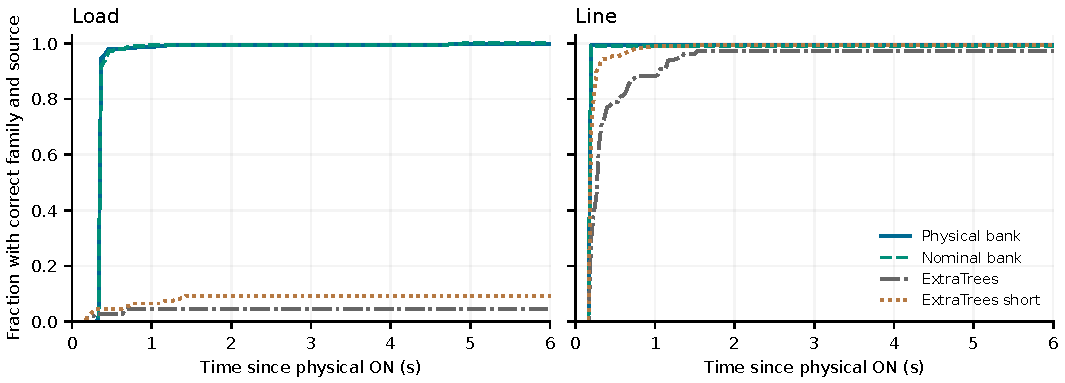
\includegraphics[width=.92\textwidth]{figures/generated/diagnosis_delay_distribution.pdf}
\caption{Distribution of correct diagnosis time, using all 324 replays per
true family in each denominator. An incorrect or absent diagnosis
contributes no mass, and late correct decisions are included, so the
curves differ from the before-OFF endpoint.}
\label{fig:diagnosis-time}\end{figure*}

\begin{figure*}[!t]\centering
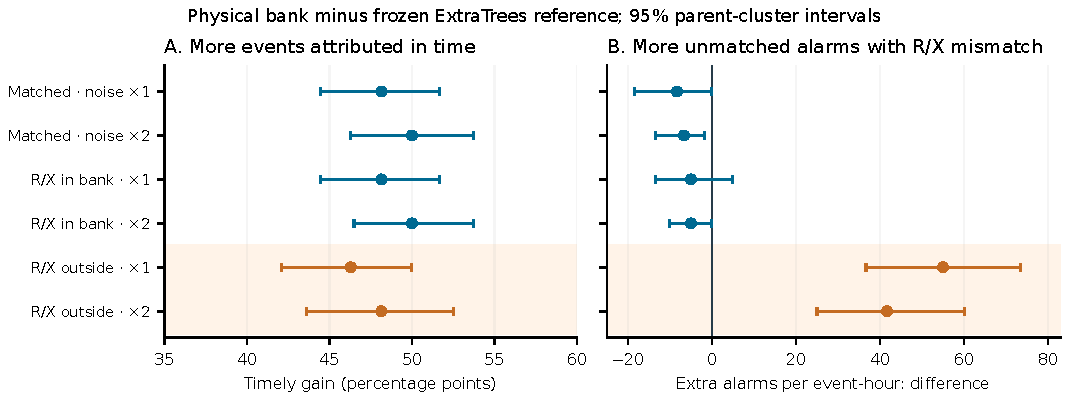
\includegraphics[width=.89\textwidth]{figures/generated/reader_c01_intervals.pdf}
\caption{Physical bank minus the ExtraTrees reference in the six paired
strata. Points and 95\% intervals come from 10{,}000 physical-parent
resamples. Left: percentage-point difference in timely attribution; right:
difference in unmatched alarms per monitored event-record hour (the 12-s
startup is excluded). Orange rows mark out-of-bank R/X conditions.}
\label{fig:c01-ci}\end{figure*}

\begin{figure*}[!t]\centering
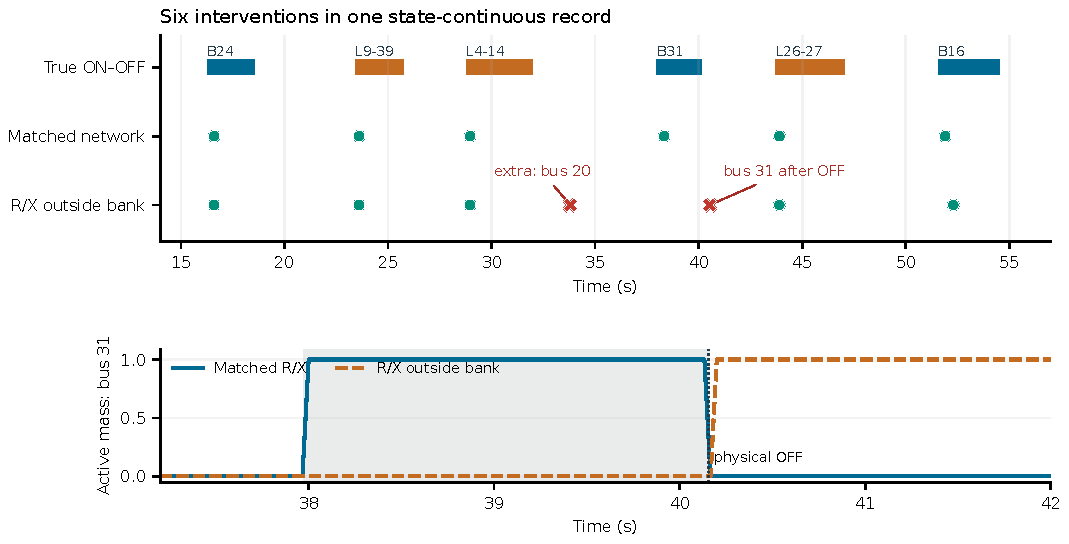
\includegraphics[width=.94\textwidth]{figures/generated/reader_episode_story.pdf}
\caption{One continuous development trajectory, shown for interpretation.
Top: physical ON--OFF intervals and emitted diagnoses under matched and
out-of-bank R/X. Bottom: bus-31 active mass with the true intervention
shaded. A diagnosis after OFF misses the timely endpoint even when it
identifies the source. True timing enters only this retrospective display.}
\label{fig:reader-story}\end{figure*}

